\documentclass[11pt]{beamer}

\usetheme{Madrid}


\usepackage[utf8]{inputenc}
\usepackage[spanish]{babel}
\usepackage{amsmath}
\usepackage{amsfonts}
\usepackage{amssymb}
\usepackage{graphicx}
\usepackage{textpos}
\usepackage{bbold}
\usepackage{physics}
\usepackage{array}



\newcommand{\p}{\ket{\psi_i}}
\newcommand{\R}{\rho}

%\renewcommand{\psi}{\ket{\psi}}

\title[Mapeos proyectivos]{Mapeos proyectivos
en sistemas de varios qubits}
\subtitle{VI Congreso Estudiantil de Física y Matemática}
\author[J. A. de León]{J. A. de León\inst{1}\and
											 C. Pineda\inst{2}\and
											 D. Dávalos\inst{2} \and
											 A. Fonseca\inst{2}\\
											 \and
											 J. D. Chang\inst{1}}
\setbeamercovered{transparent} 
\setbeamertemplate{navigation symbols}{} 
%\logo{\includegraphics[height=1.5cm]{logoECFM.png}\vspace{0.5pt}} 
\institute[ECFM-USAC]{
	\inst{1}
	Escuela de Ciencias Físicas y Matemáticas\\
	USAC
	\and
	\inst{2}
	Instituto de Física\\
	UNAM} 
\date[VI Congreso Estudiantil]{Septiembre 2020} 
 

\begin{document}

\begin{frame}
\titlepage
\end{frame}

\addtobeamertemplate{frametitle}{}{%
\begin{textblock*}{100mm}(.90\textwidth,6.9cm)
%\includegraphics[height=1.2cm]{logoECFM.png}
\end{textblock*}}

\begin{frame}{Esquema}
\tableofcontents
\end{frame}

\AtBeginSubsection[]
{
\begin{frame}[noframenumbering]
\tableofcontents[currentsection, currentsubsection]
\end{frame}
}

\AtBeginSection[]
{
\begin{frame}[noframenumbering]
\tableofcontents[currentsection]
\end{frame}
}

\begin{frame}{Motivación}
	\centering
	\LARGE
	estados físicos $\underset{\text{proceso físico}
  }{\mbox{\Huge $\longmapsto$}}$ otros estados físicos
\end{frame}

\section[Hola]{Marco teórico}
\subsection{Qubits}
\begin{frame}{Bits}
La arquitectura de las computadoras convencionales la constituyen
microprocesadores que están construidos con millones de transistores.\vfill

Un transistor puede estar
\begin{columns}
	\begin{column}{0.5\textwidth}
		\begin{center}
		\begin{tabular}{rl}
			encendido = & 1, \\ 
			apagado = & 0.
		\end{tabular} 
		\end{center}
	\end{column}
	\begin{column}{0.5\textwidth}
		\begin{figure}[H]
			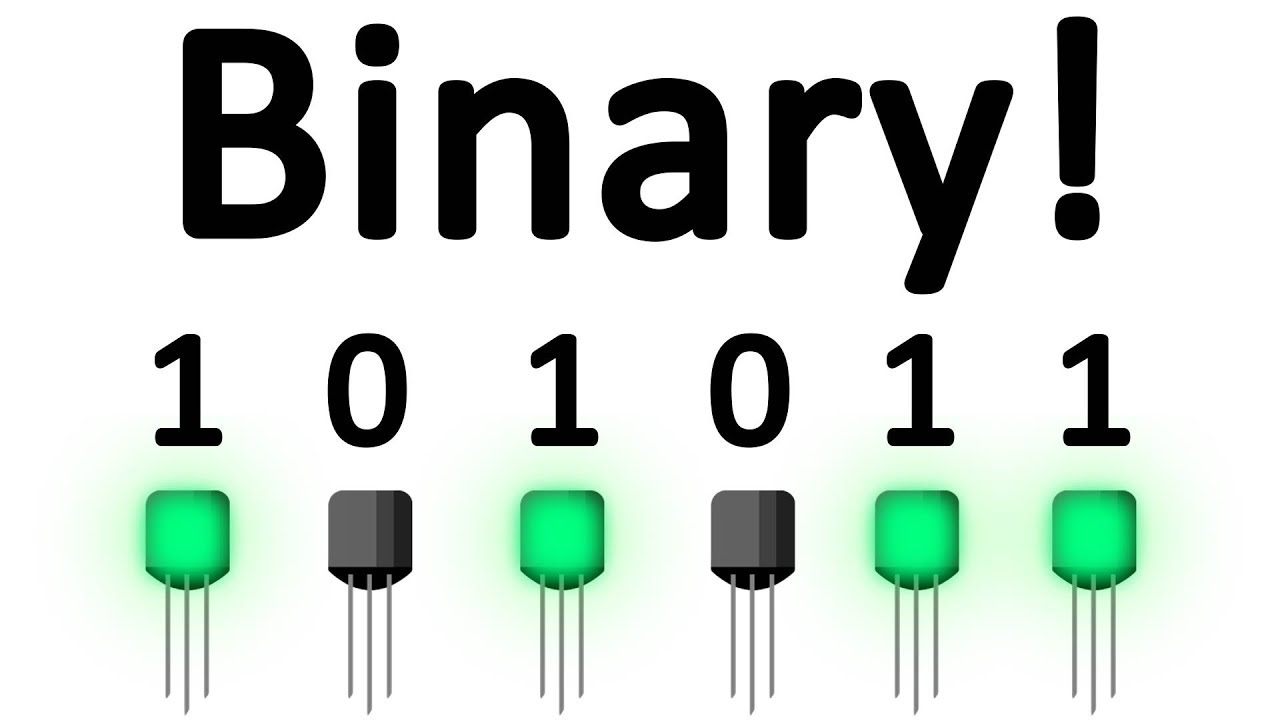
\includegraphics[width=0.9\textwidth]{img-congreso/bits.jpg}
		\end{figure}
	\end{column}
\end{columns}\vfill

Haciendo operaciones lógicas con los bits funcionan 
las computadoras de hoy. 
\end{frame}


\begin{frame}{Qubits}
\vfill
Las computadoras cuánticas procesan información utilizando 
\textbf{bits cuánticos}. Debido a su naturaleza cuántica,los \textbf{qbits} 
pueden estar encendidos y apagados al mismo tiempo. \vfill

El estado de un qubit se representa por medio de 
un vector $\ket{\psi}$ en un espacio vectorial complejo de Hilbert 
$\mathcal{H}$ (espacio de estados, $\mathbb{C}^2$),
\begin{equation}
	\ket{\psi} = \alpha \ket{0} + \beta \ket{1}, \hspace{25pt}
	\alpha, \beta \in \mathbb{C},
	\hspace{25pt} \abs{\alpha}^2 + \abs{\beta}^2 = 1.
\end{equation} \vfill
\end{frame}

\begin{frame}{Sistema de varios qubits}
	\vfill
	El espacio de estados total $\mathcal{H}_\text{total}$ de un sistema de 
	$n$ qubits es
	el producto tensorial de los espacios individuales $\mathcal{H}_i$
	de cada uno de 	los qubits,
	\begin{equation}
		\mathcal{H}_{\text{total}} = \underbrace{\mathbb{C}^2 \otimes 
		\mathbb{C}^2 \otimes \mathbb{C}^2 \otimes 
		\cdots \otimes \mathbb{C}^2}_{n \text{ veces}},
	\end{equation}
	donde $\dim \mathcal{H}_{\text{total}} = 2^n$. \vfill
\end{frame}

\begin{frame}{Qubits}
Implementaciones físicas:
\begin{itemize}
	\item Espín de un electrón
	\item Fotón polarizado
	\item Red óptica
	\item Puntos cuánticos
	\item ... cualquier sistema cuántico de dos niveles.
\end{itemize}\vfill

**poner alguna imagen amigable del espín 1/2
\end{frame}

\begin{frame}
¿Qué consecuencias tiene utilizar las reglas de la mecánica cuántica para
procesar información?
	\begin{align*}
		231654687498461 = ? \times ?
	\end{align*}\vfill
	Peter Shor, en 1994, mostró que problemas difíciles en el mundo clásico son
	problemas fáciles en el mundo cuántico. \vfill
	\begin{columns}
	\begin{column}{0.5\textwidth}
		\vfill
  	\begin{center}
  		\textbf{Computadora clásica:}
  	\end{center}
  	\begin{itemize}
  		\item Factorizar un número de 193 dígitos tomó 30 años de CPU (2.2 GHz). 
  		\item Factorizar un número de 500 dígitos tomaría $10^{12}$ años de CPU.
  	\end{itemize}
	\end{column}
	\begin{column}{0.5\textwidth}  %%<--- here
  	\begin{center}
  		\textbf{Computadora cuántica:}
  	\end{center}
  	\begin{itemize}
  		\item Se podría factorizar un número de 193 dígitos en 0.1 s. 
  		\item Se podría factorizar un número de 500 dígitos en 2 s. 
  	\end{itemize}
  	\vspace{15pt}
	\end{column}
	\end{columns}\vfill
	\vspace{20pt}
	A esta propiedad John Preskill, en el 2012, le llamó 
	\textbf{supremacía cuántica}. \vfill
\end{frame}

\begin{frame}{Ventajas del mundo cuántico}
	\begin{itemize}
		\item \textbf{Aleatoriedad}: no se puede predecir el resultado de una 
						medición aún con la descripción más completa de un estado cuántico.
						Esta propiedad es intrínseca.
		
		\item \textbf{Incertidumbre}: esta propiedad es inherente de la teoría y 
						no puede ser eliminada buscando más información.
		
		\item \textbf{Entrelazamiento}: aún con la descripción más completa de un
									sistema compuesto $AB$ la conocimiento sobre estado de un 
									subsistema podría ser incompleto. 
	\end{itemize}\vfill
	
	\emph{`El entrelazamiento no es una sino la característica de la
	mecánica cuántica.' - E. Schrödinger.}
\end{frame}



\subsection{Matriz de densidad}
\begin{frame}{Ensambles de estados cuánticos}
Dada la incertidumbre intrínseca de la mecánica cuántica tenemos que 
enfrentarnos a dos escenarios: 
\begin{enumerate}
	\item \textbf{Ignorancia}: simplemente desconocemos cuál es el estado cuántico del 
				sistema.
	\item \textbf{Muchas posibilidades}: un sistema puede estar en muchos estados, en uno
				del \textbf{ensamble de estados} $\{ p_i, \p \}$.
\end{enumerate} \vfill

Por ejemplo, 1 qubit podría estar en alguno de los estados en el ensamble
$\{ p_0,\ket{0}; p_1, \ket{1} \}$.\vfill

En cualquiera de los dos contextos se puede utilizar el mismo formalismo:
la \textbf{matriz de densidad}. 
\end{frame}



\begin{frame}{La matriz de densidad}
Si un sistema cuántico se encuentra en alguno de los estados del ensamble
$\{ p_i, \ket{\psi _i} \}$, entonces la matriz de densidad
$\rho$ del sistema es
\begin{equation}
	\rho = \sum _i p_i\dyad{\psi_i}{\psi_i}.
\end{equation}
\end{frame}


\begin{frame}{La matriz de densidad}
Es útil y conveniente optar por una definición de la matriz de densidad
independiente a la de la descripción de un ensamble de estados. \vfill

\textbf{Caracterización de las matrices de densidad:}
Una matriz compleja $\R$, que actúa sobre un espacio de Hilbert
$\mathcal{H}$, es una matriz de densidad si y sólo si 

\begin{center}
\begin{tabular}{ll}
(i) Hermítica, & $\rho = \rho ^{\dagger}$, \\ 
(ii) positiva, & $\rho \geq 0$, \\ 
(iii) normalizada, & $\Tr \rho = 1$. \\ 

\end{tabular} 
\end{center}
\vfill
\end{frame}

\begin{frame}{La esfera de Bloch}
Una matriz de densidad $\rho$ arbitraria de un qubit se puede escribir como
\begin{equation}
	\rho = \frac{\mathbb{1} + \vec{r}\vdot \vec{\sigma}}{2}, 
\end{equation}
donde $\vec{r}$ es un vector en una esfera de unitaria, llamada la
\textbf{esfera de Bloch}, tal que $\norm{
\vec{r}} \leq 1$ y $\vec{\sigma}$ es un 
vector con las matrices de Pauli en sus entradas,
\begin{align*}
	\sigma _x &= \mqty(0&1 \\ 1&0), &
	\sigma _y &= \mqty(0&-i \\ i&0), &	
	\sigma _z &= \mqty(1&0 \\ 0&-1).
\end{align*}

\begin{equation}
	\rho = \mqty(1 + r_z & r_x - ir_y \\
								r_x + ir_y & 1 - r_z). 
\end{equation}
\end{frame}


\begin{frame}{La esfera de Bloch}
\begin{figure}
	\centering
	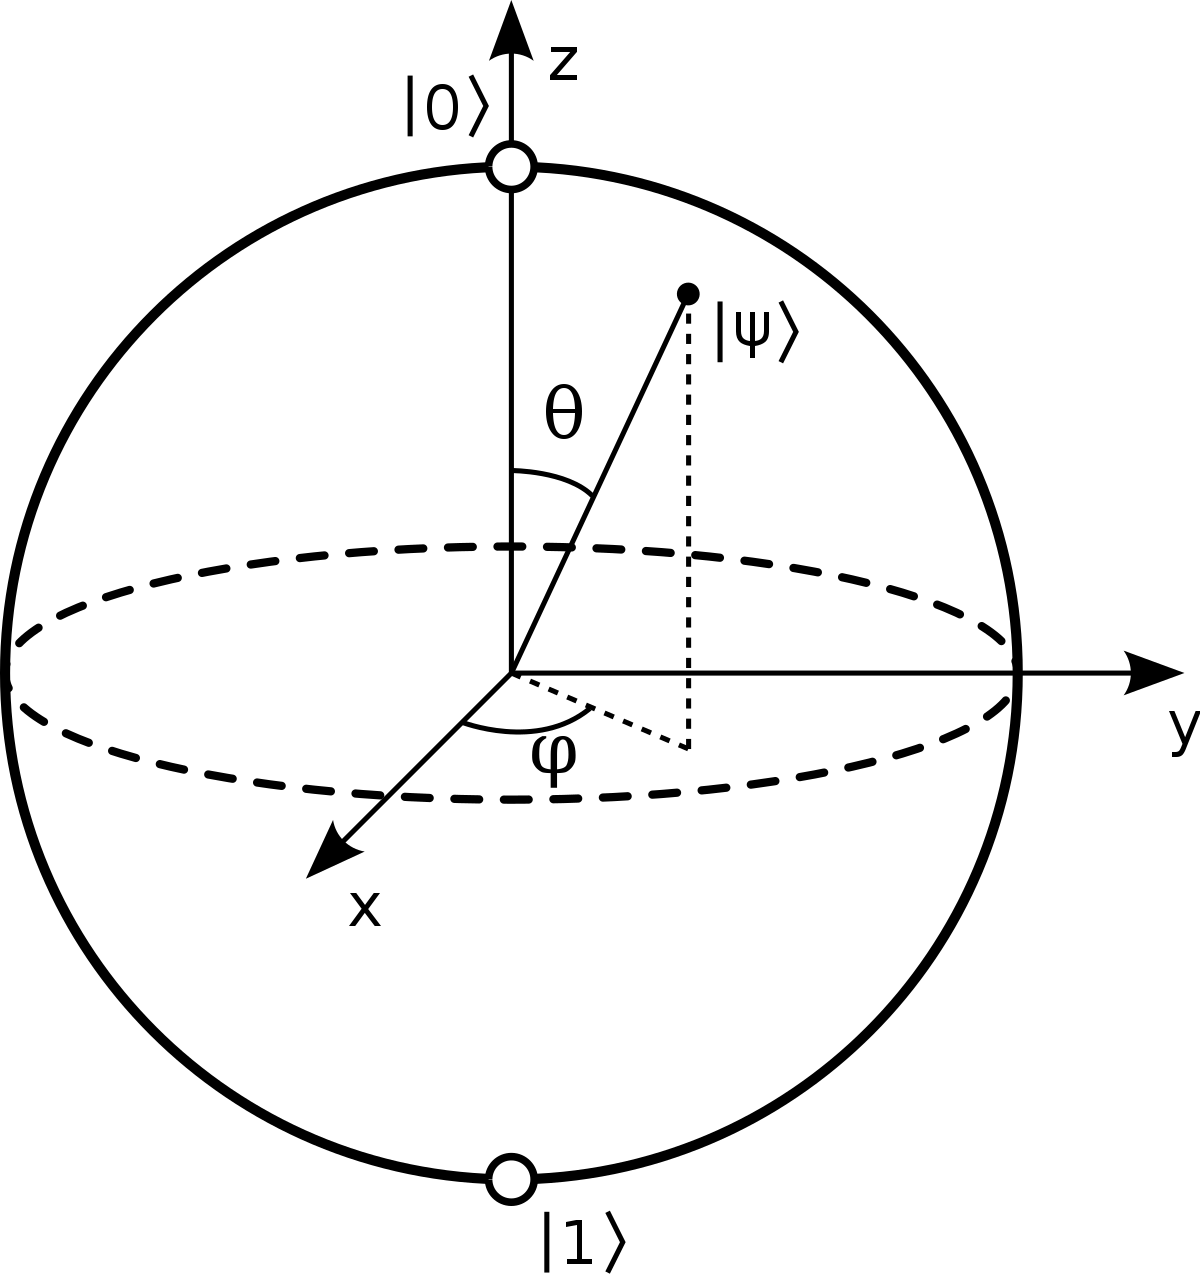
\includegraphics[height=0.5\textheight]{img-congreso/blochSphere.pdf}
	\caption{El estado de un qubit tiene representación como un punto en la
	esfera de Bloch.}
\end{figure}
\end{frame}


\begin{frame}{$\rho$ de $n$ qubits}
	En ese sentido, una matriz de densidad arbitraria de $n$ qubits puede 
	escribirse como
	\begin{equation}
		\rho = \sum _{\vec{v}}\frac{\Tr \qty(\sigma _{v_1} \otimes \sigma _{v_2} 
		\otimes 
		\cdots \otimes \sigma _{v_n} \rho)
		\sigma _{v_1} \otimes \sigma _{v_2} \otimes 
		\cdots \otimes \sigma _{v_n}}{2^n},
	\end{equation}
	donde la sumatoria va sobre los vectores $\vec{v}=\qty(v_1, v_2, \ldots, v_n)$
	con entradas $v_i$ seleccionados del conjunto $\{0,1,2,3\}$. \vfill
	
	Conviene	interpretar a los coeficientes
	$\Tr \qty(\sigma _{v_1} \otimes \sigma _{v_2} 
	\otimes \cdots \otimes \sigma _{v_n} \rho)$ 
	como las $2^{2n}-1$ componentes de un vector $\vec{r}$ en la hiperesfera 
	de Bloch.
\end{frame}

\subsection{Canales cuánticos}

\begin{frame}{Sistemas cuánticos abiertos}
Se dice que un sistema cuántico es cerrado cuando este no interactúa con su
entorno. Por el otro lado, un sistema que sí interactúa con su 
entorno se conoce como \textbf{sistema cuántico abierto}. \vfill

A diferencia de los sistemas cuánticos cerrados, la dinámica de los sistemas
cuánticos abiertos no se puede describir con operadores unitarios. Por ello,
una herramienta para hacerlo es el formalismo
de los \textbf{canales cuánticos}. 
\end{frame}

\begin{frame}{Canales cuánticos}
Un estado cuántico se transforma como
\begin{align}
	\rho ' = \Phi \qty(\rho),
\end{align}
donde $\Phi$ es un \textbf{canal cuántico}. El canal cuántico $\Phi$
permite describir el cambio dinámico de un estado cuántico $\rho$ 
que ocurre como resultado de un proceso físico; $\rho$ es el estado inicial
y $\rho'$ el estado final luego de ocurrir el proceso.
\end{frame}

\begin{frame}{Canales cuánticos}
Para que $\Phi$ sea un canal cuántico, debe
\begin{enumerate}
	\item ser lineal,
	\item preservar $\Tr \rho$,
	\item ser completamente positivo.
\end{enumerate}\vfill
¿Completamente positivo? 
\end{frame}


\begin{frame}{Completa positividad}
	El estado $\rho$ de un sistema puede ser extendido por una \emph{ancilla}
	$\sigma$, el estado de cualquier otro sistema cuántico. Por ello, no es
	suficiente que $\Phi (\rho)$ sea una matriz de densidad válida; es 
	necesario que $\Phi (\rho) \otimes \sigma$ también lo sea para cualquier
	estado $\sigma$.\vfill
	
	Dicho de otro modo, $\Phi$ es completamente positivo si y sólo si para una
	extensión dimensional arbitraria $K$
	\begin{align*}
		\mathcal{H}_n \rightarrow \mathcal{H}_n\otimes \mathcal{H}_K
	\end{align*}
	el mapeo $\Phi\otimes \mathbb{1}_K$ es positivo.
\end{frame}


\section{Mapeos proyectivos en sistemas de varios qubits}
\subsection{Motivación}
\begin{frame}{Información Cuántica}
  ¿Es posible manipular y controlar sistemas cuánticos complejos?
	
	Si es así, ¿qué implicaciones científicas	y tecnológicas tiene eso?
\end{frame}

\begin{frame}
¿Será que colapsar una dimensión en la esfera de Bloch de un qubit 
representa un proceso físico? \vfill

*un dibujo bien chilero de eso*
\end{frame}


\begin{frame}
¿Cómo se modifica la matriz de densidad de un qubit ante una acción como esa?

\begin{figure}[H]
\centering
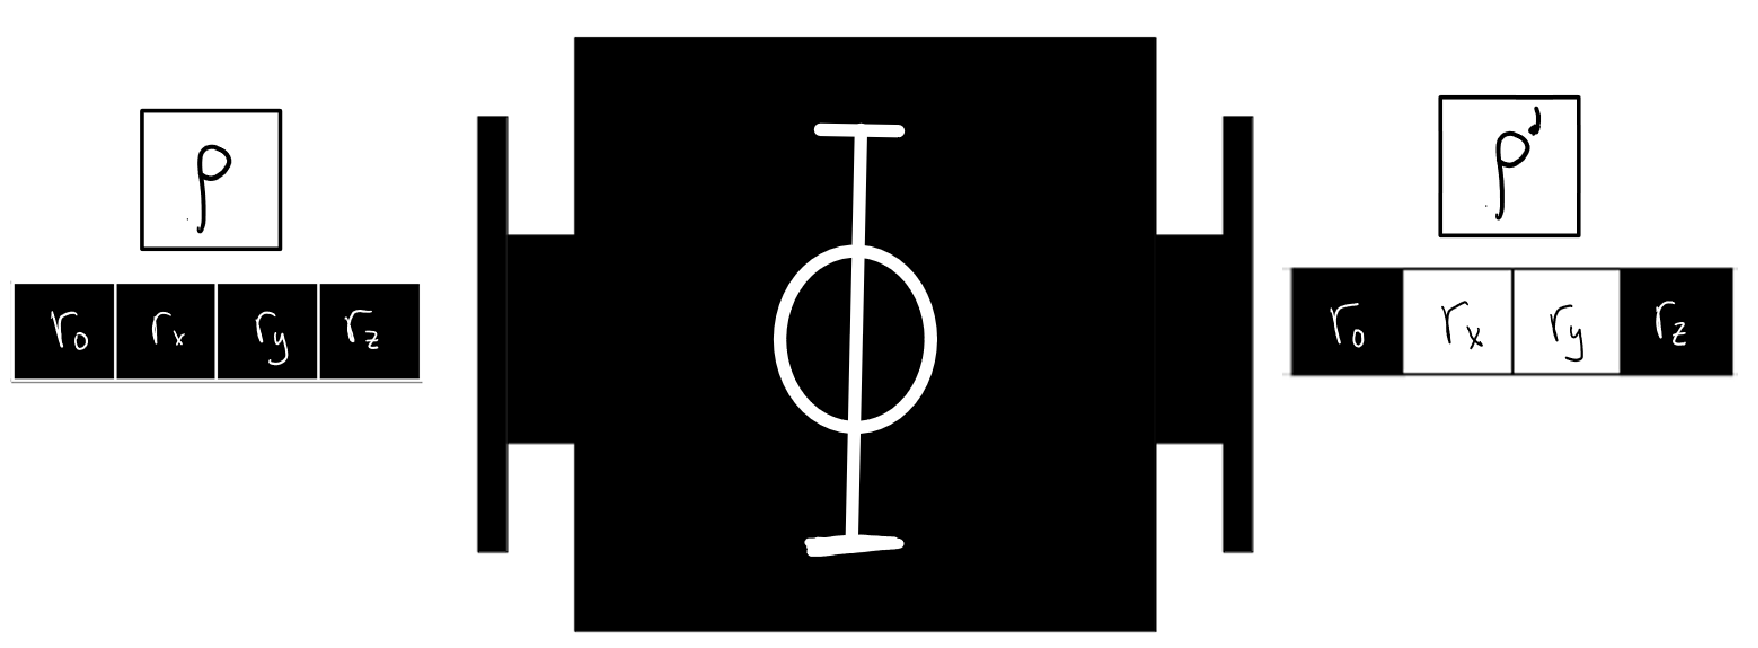
\includegraphics[width=0.9\linewidth]{img-congreso/ja.pdf}
\label{fig:1qubit-draw}
\caption{Representación gráfica de la acción de un mapeo de 1 qubit que 
mantiene invariantes dos componentes ($r_0$ y $r_z$) y borra dos 
componentes ($r_x$ y $r_y$) de la matriz de densidad inicial $\rho$.}
\end{figure}

\end{frame}


\begin{frame}
Si ahora consideramos el caso de 2 qubits sería imposible imaginar una
hiperesfera de 15 dimensiones, pero podemos utilizar la siguiente 
representación de la matriz de densidad.
\begin{figure}[H]
\centering
  \caption{Representación gráfica de la matriz de densidad de 2 qubits.}
  \begin{minipage}{0.5\textwidth}
  	\centering
  	\vspace{22pt}
    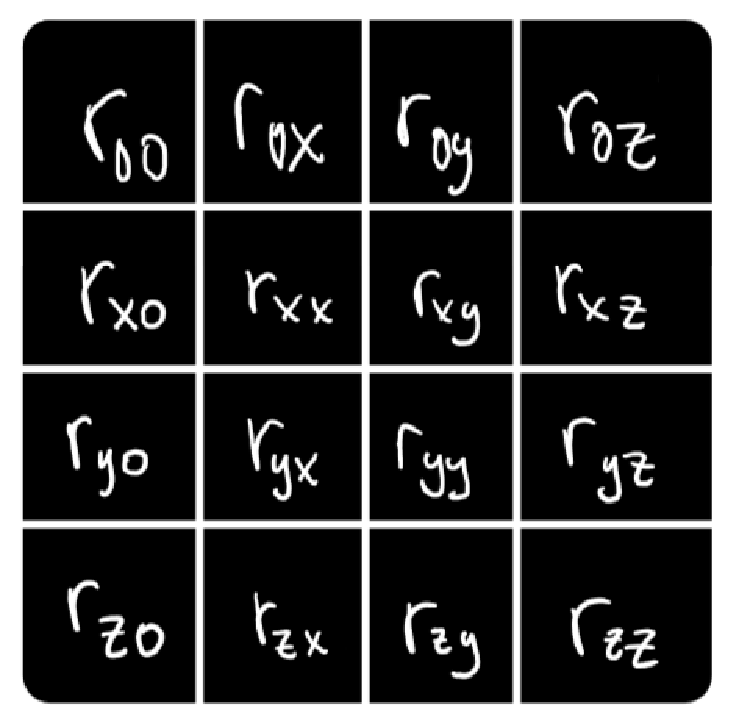
\includegraphics[width=0.625\textwidth]{img-congreso/rho2q.pdf}
    \vspace{20pt}
  \end{minipage}\hfill
  \begin{minipage}{0.5\textwidth}
  	\centering
    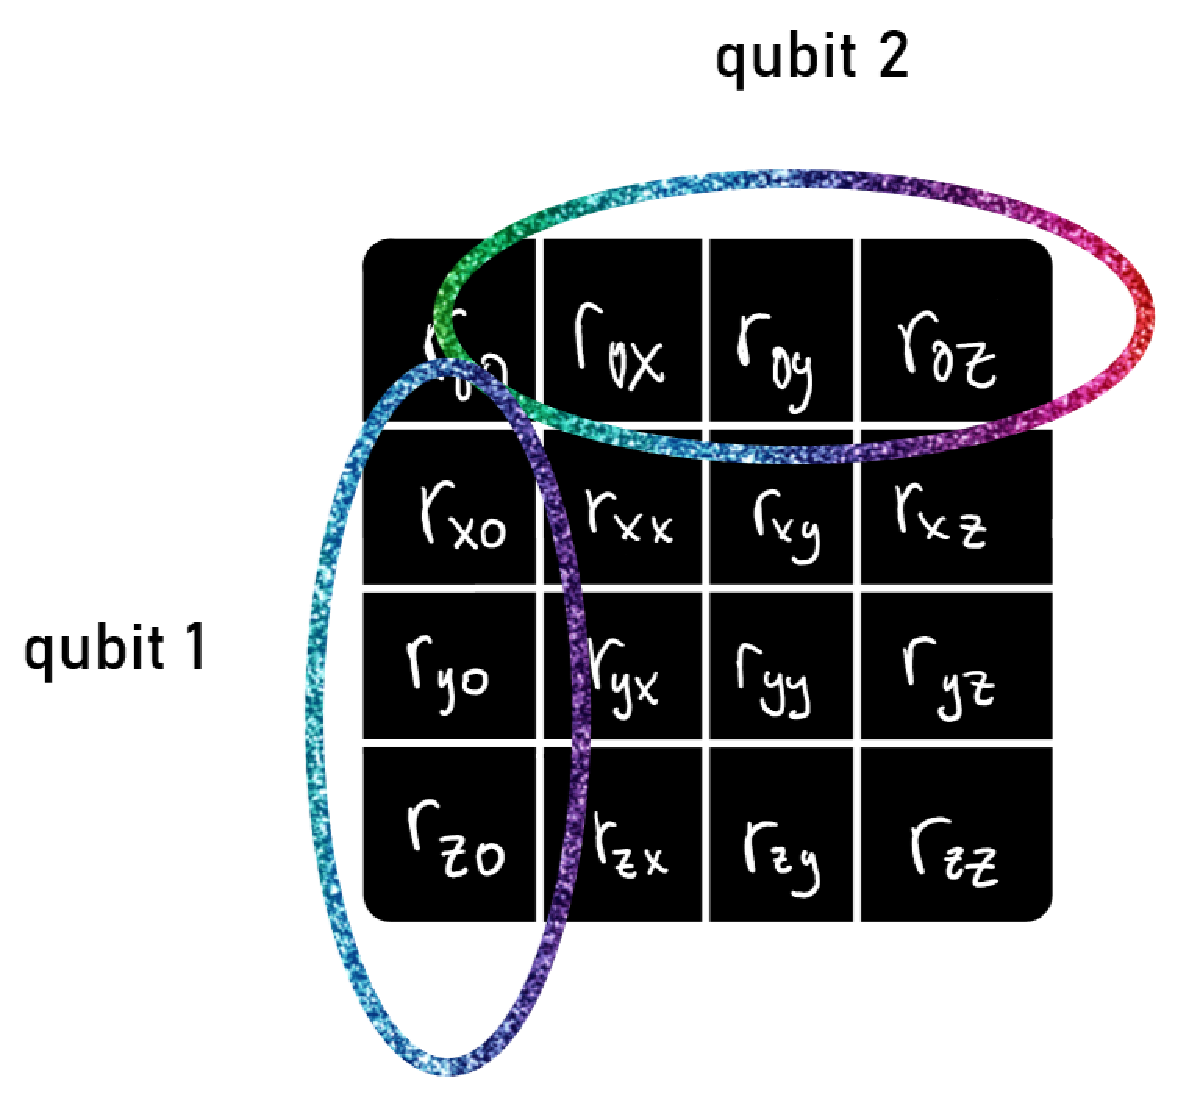
\includegraphics[width=\textwidth]{img-congreso/rho2q(1).pdf}
  \end{minipage}
\end{figure}

\end{frame}


\begin{frame}

\begin{figure}[H]
\centering
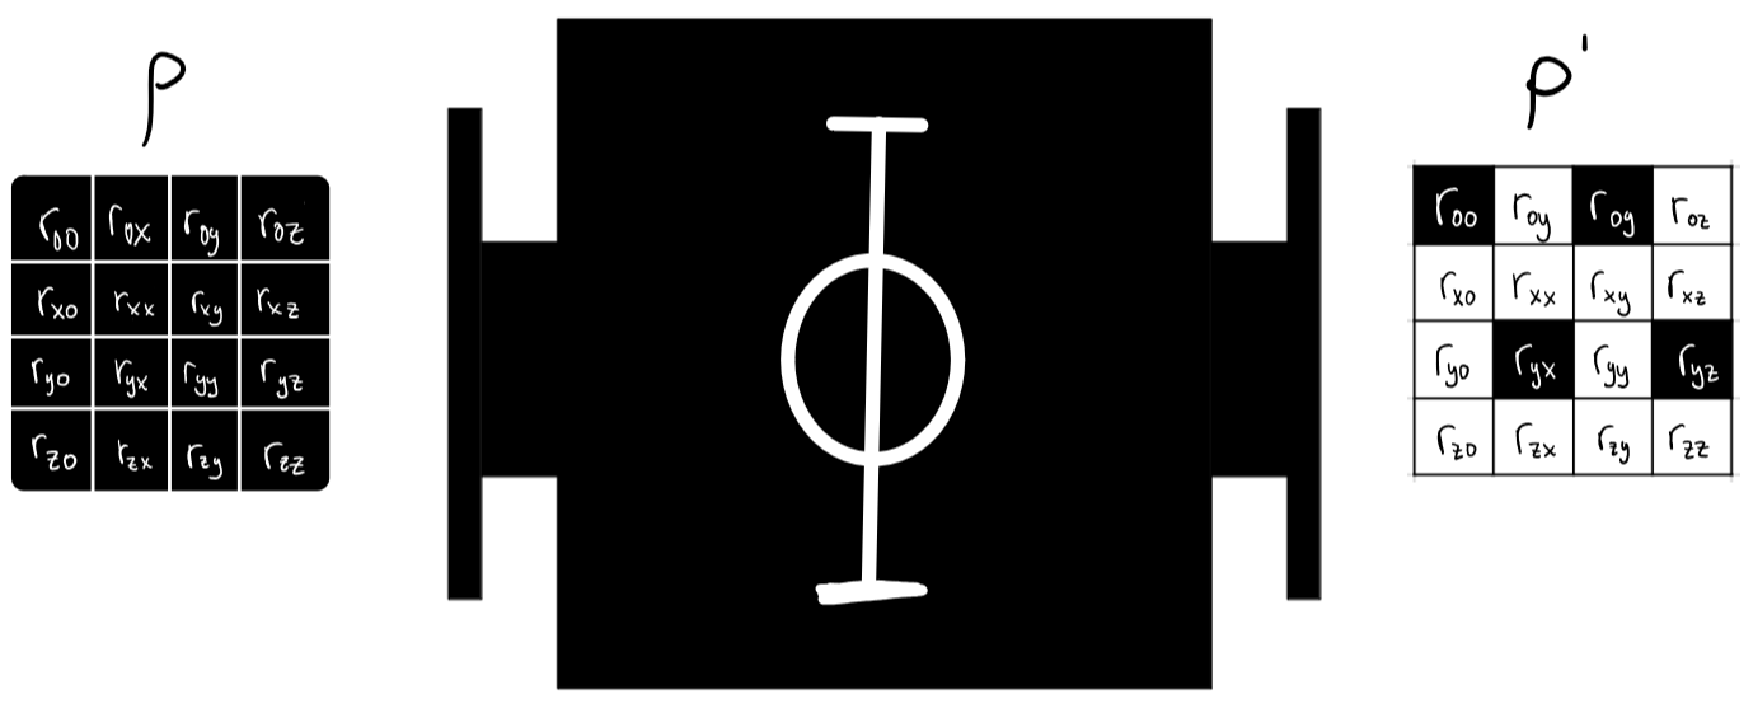
\includegraphics[width=0.9\linewidth]{img-congreso/2qubits.pdf}
\label{fig:1qubit-draw}
\caption{Representación gráfica de la acción de un mapeo de 2 qubits que mantiene invariantes 4 componentes y borra 12 componentes de la matriz de densidad inicial $\rho$.}
\end{figure}

\end{frame}

\subsection{Planteamiento del problema}
\begin{frame}{Planteamiento del problema}
	En un sistema de $n$ qubits, ¿qué componentes se pueden borrar de 
	la matriz de densidad y que éste sea un proceso físico?
\end{frame}

\section{Resultados}

\subsection{1 qubit}
\begin{frame}{1 qubit}
Se tienen 8 mapeos posibles. *colocar imagen de los cuadritos*
\end{frame}

\begin{frame}{1 qubit}
\begin{figure}[H]
\centering
\caption{Representación de las matrices de densidad resultantes de
los mapeos válidos de 1 qubit.}
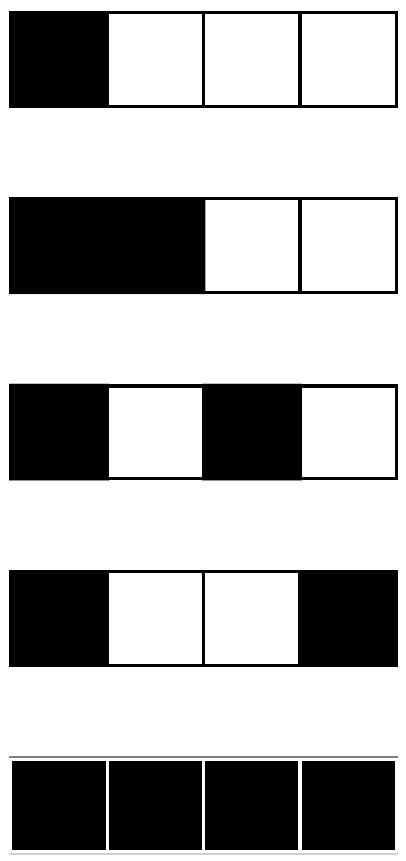
\includegraphics[height=0.35\textheight]{img-congreso/1qubit-CCs.pdf}
\label{fig:1qubit-CCs}
\end{figure}

En conclusión, para 1 qubit son canales cuánticos los mapeos que colapsan 0,
2 y 3 dimensiones de la esfera de Bloch (o bien, dejan invariantes 0, 2 y 4
componentes). \vfill

¿Será que, en general, son válidos los mapeos que borran $2^{2n} - 2^j$, con
$j = 0, 1, \ldots, \dim \mathcal{H}$?\vfill
\end{frame}


\subsection{2 qubits}
\begin{frame}{2 qubits}
	Hay 15 parámetros que se pueden mantener invariantes o borrar, entonces
	hay $2^{15} = 32,768$ posibles mapeos. *colocar imagen de algunos cuadritos* 
\end{frame}

\begin{frame}{2 qubits, 2 componentes invariantes:}

\begin{figure}[H]
\centering
  \begin{minipage}{0.8\textwidth}
  	\centering
    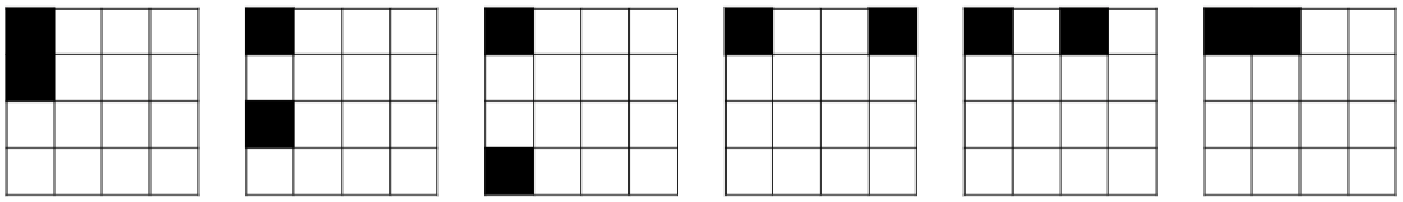
\includegraphics[width=\textwidth]{img-congreso/C12.pdf}
    \caption{Clase de equivalencia $C_1^2$.}
  \end{minipage}\vfill
  \begin{minipage}{0.8\textwidth}
  	\centering
    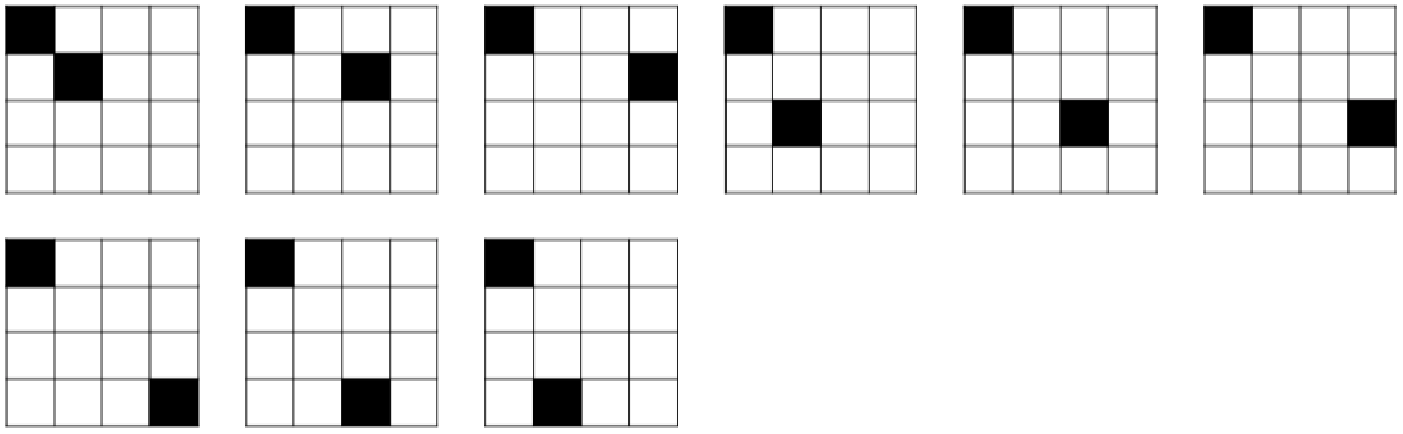
\includegraphics[width=\textwidth]{img-congreso/C22.pdf}
    \caption{Clase de equivalencia $C_2^2$.}
  \end{minipage}
\end{figure}\vfill
Mapeos posibles = $15 \choose 1$ = 15. Canales cuánticos = 15.

\end{frame}



\begin{frame}{2 qubits, 4 componentes invariantes:}

\begin{figure}[H]
\centering
  \begin{minipage}{0.48\textwidth}
  	\centering
  	\vspace{30pt}
    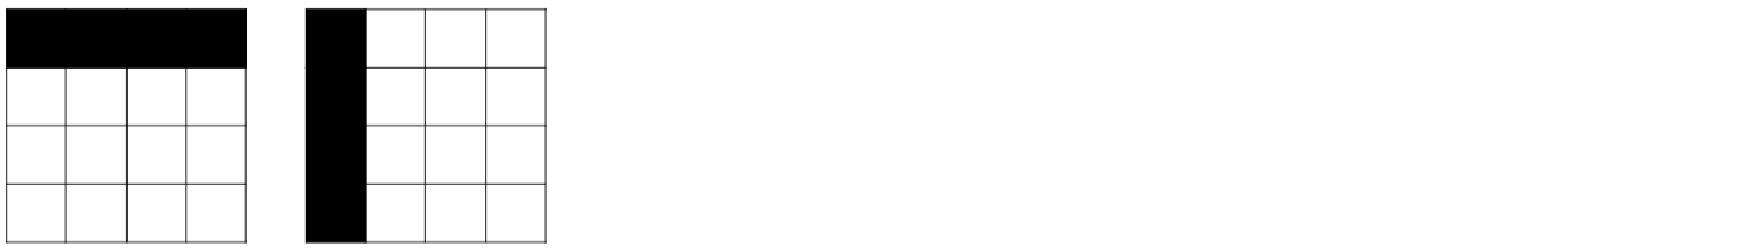
\includegraphics[width=\textwidth]{img-congreso/C14.pdf}
    \caption{Clase de equivalencia $C_1^2$.}
  \end{minipage}\hfill
  \begin{minipage}{0.48\textwidth}
  	\centering
    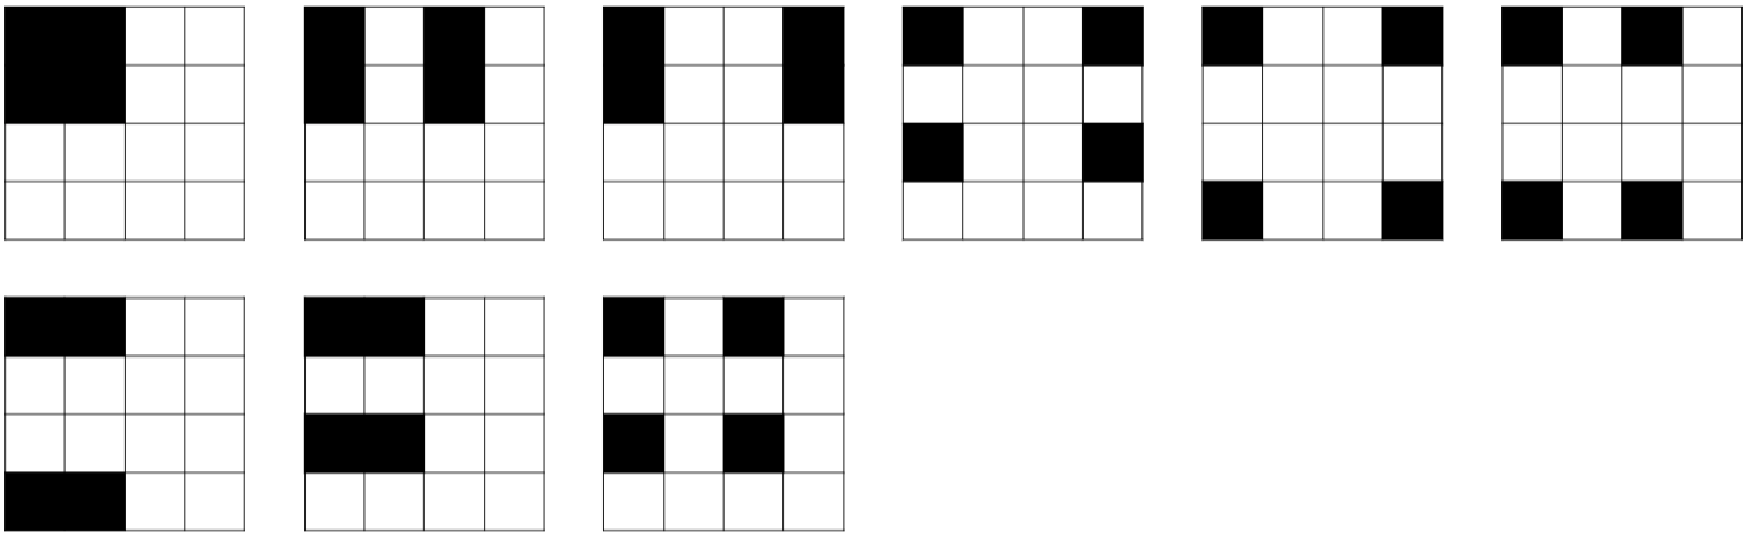
\includegraphics[width=\textwidth]{img-congreso/C24.pdf}
    \caption{Clase de equivalencia $C_2^2$.}
  \end{minipage}\vfill
  
  \begin{minipage}{0.48\textwidth}
  	\centering
    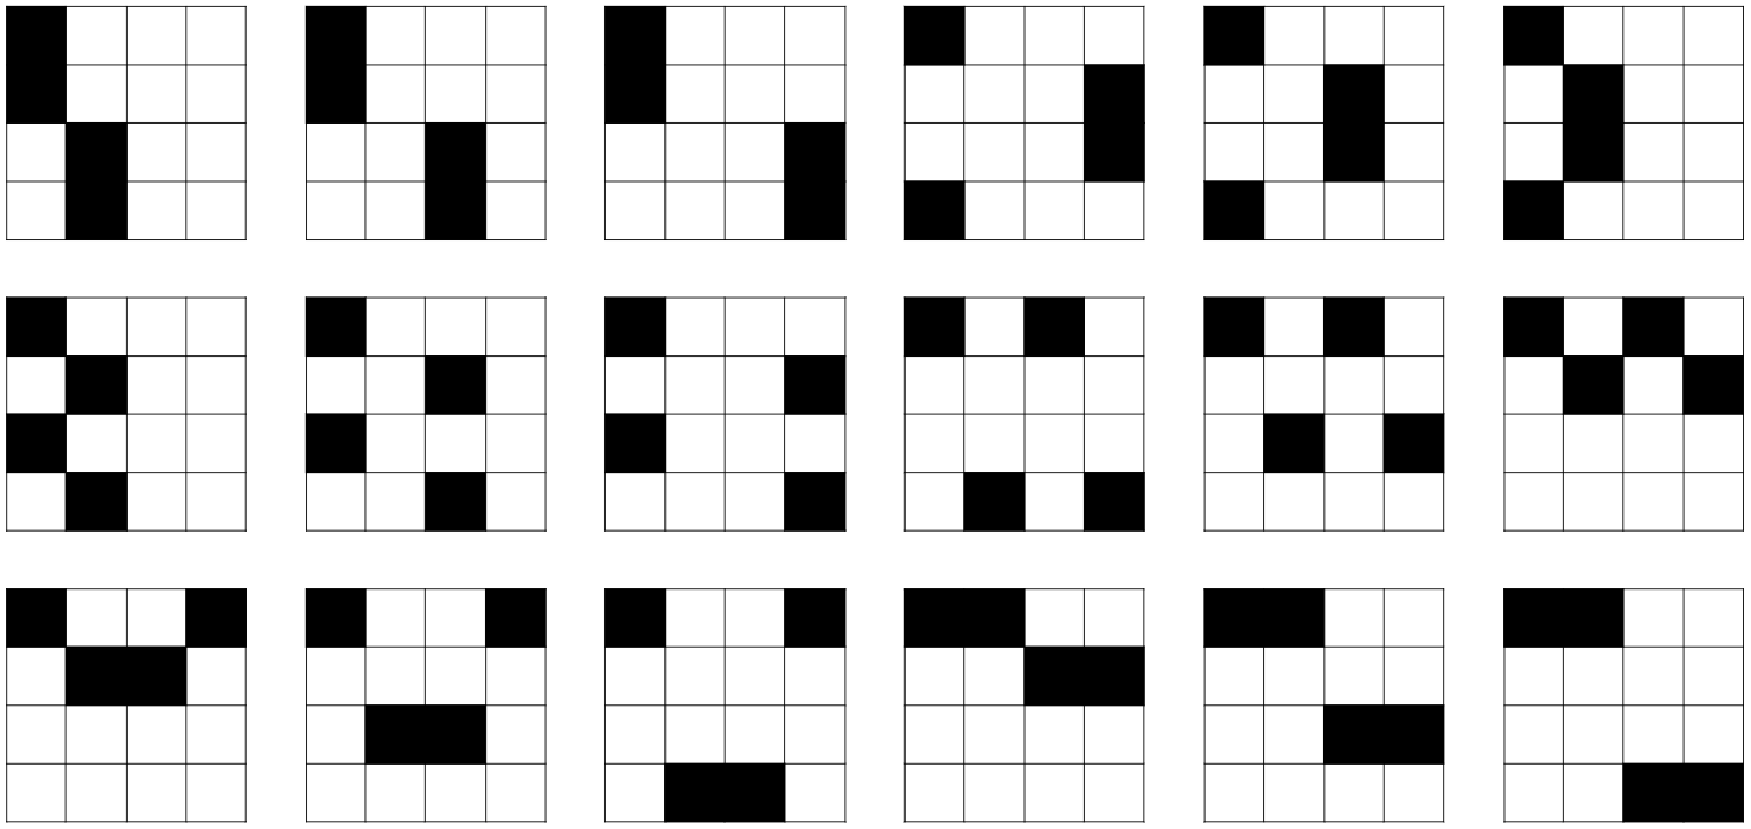
\includegraphics[width=\textwidth]{img-congreso/C34.pdf}
    \caption{Clase de equivalencia $C_1^2$.}
  \end{minipage}\hfill
  \begin{minipage}{0.48\textwidth}
  	\centering
  	\vspace{50pt}
    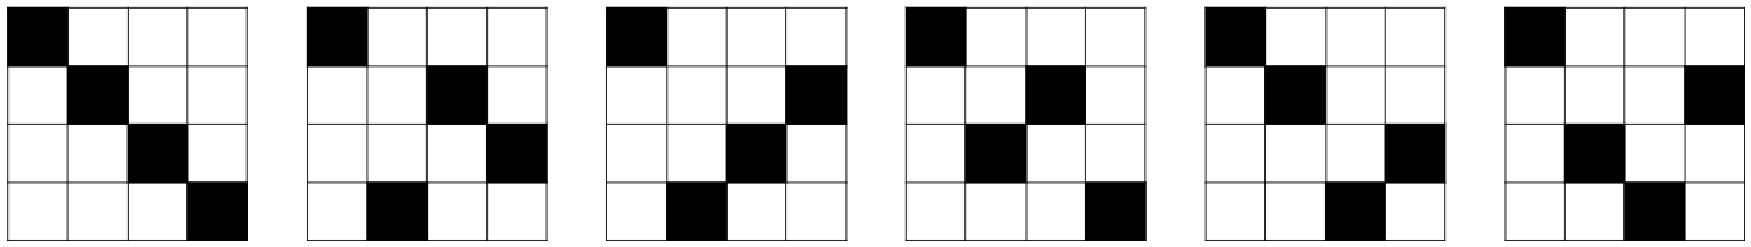
\includegraphics[width=\textwidth]{img-congreso/C44.pdf}
    \caption{Clase de equivalencia $C_2^2$.}
  \end{minipage}
\end{figure}\vfill
Mapeos posibles = $15 \choose 3$ = 455. Canales cuánticos = 35.

\end{frame}



\begin{frame}{2 qubits, 8 componentes invariantes:}

\begin{figure}[H]
\centering
  \begin{minipage}{0.8\textwidth}
  	\centering
    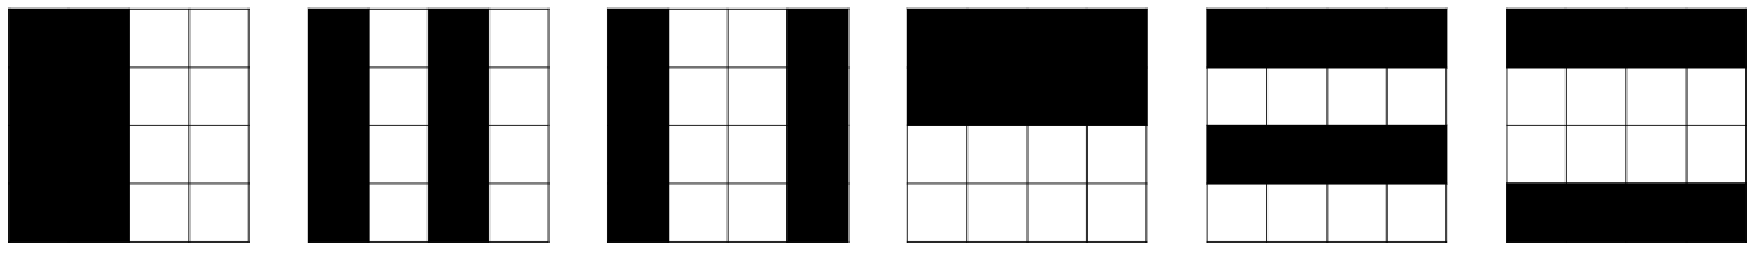
\includegraphics[width=\textwidth]{img-congreso/C18.pdf}
    \caption{Clase de equivalencia $C_1^8$.}
  \end{minipage}\vfill
  \begin{minipage}{0.8\textwidth}
  	\centering
    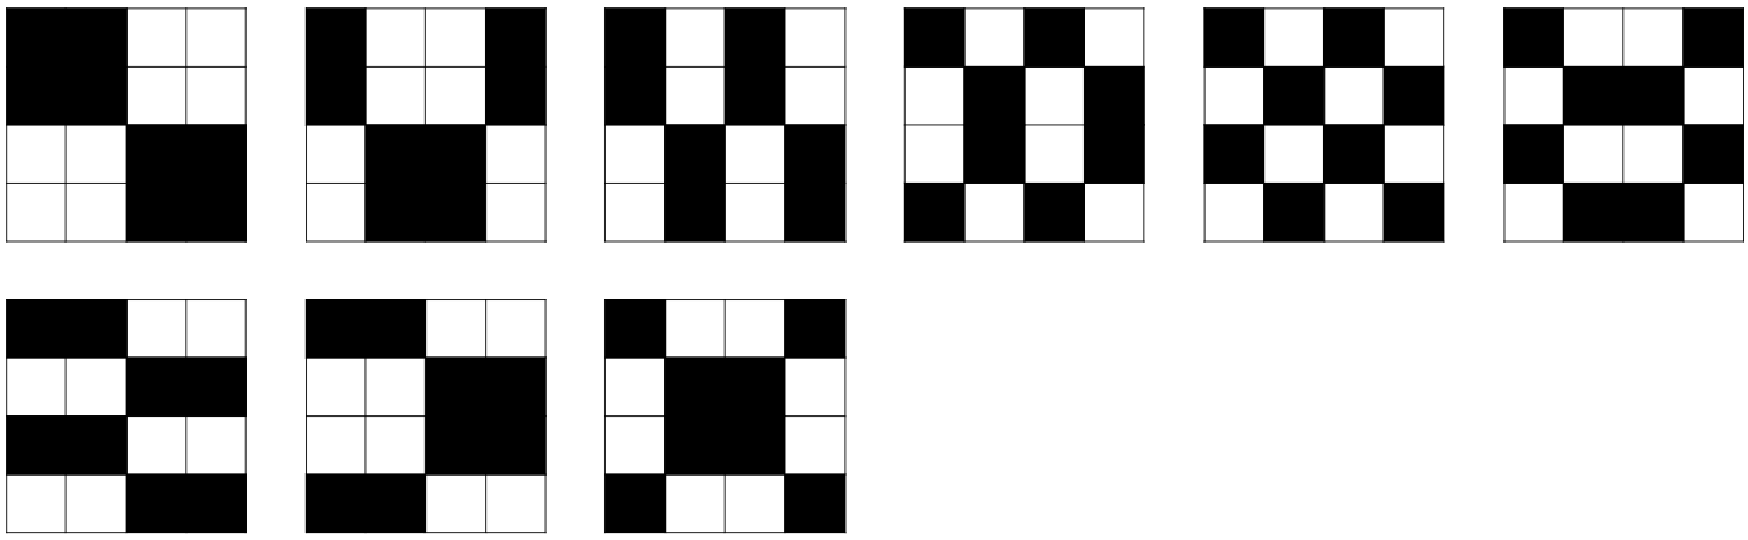
\includegraphics[width=\textwidth]{img-congreso/C28.pdf}
    \caption{Clase de equivalencia $C_2^8$.}
  \end{minipage}
\end{figure}
Mapeos posibles = $15 \choose 7$ = 6435. Canales cuánticos = 15.

\end{frame}

\begin{frame}
	Sobre las componentes 'individuales' de cada qubit se respetan los
	resultados de 1 qubit. \vfill
	
	Por ello, presumimos que esto debe cumplirse recursivamente conforme
	se aumenta el número de qubits en el sistema. 
\end{frame}

\begin{frame}
	¿Qué onda entonces con las clases de equivalencia? \vfill
	
	Dentro de cada clase las matrices están conectadas por transposición o
	permutaciones de las filas o columnas 1, 2 y 3. Es decir, estos mapeos
	son invariantes ante intercambio de partículas e intercambio de las
	coordenadas $x$, $y$ y $z$ de cada qubit.
\end{frame}



\begin{frame}
	Los canales cuánticos no dependen únicamente del número de componentes
	que borran de la matriz de densidad. \textbf{Si importa qué componentes
	se borren.} \vfill
	
	Número de canales válidos según el número de qubits en el sistema y el 
	número de componentes que dejan invariantes:
	\vspace{10pt}
	
	\begin{tabular}{>{$n=}l<{$\hspace{12pt}}*{13}{c}}
		1 &&&&&&1&3&1&&&&&\\
		2 &&&&&1&15&35&15&1&&&&\\
	\end{tabular}\vfill
	
	¿se podrá encontrar alguna relación para calcular el número de canales
	cuánticos por cantidad de componentes que mantienen invariantes?
\end{frame}



\begin{frame}
Si bien, la condición de borrar 
$2^{\dim\mathcal{H}} - 2^j$ componentes de $\rho$
con $j = 0, 1, \ldots, n$ no es suficiente para caracterizar a 
los mapeos de nuestro interés, los resultados apuntan que es 
una condición necesaria. 
\end{frame}

\section{Trabajo futuro}
\begin{frame}{Trabajo futuro}
	\begin{itemize}
		\item	Buscar una caracterización de las clases de equivalencia para poder
					construir una matriz que genere al resto de los elementos en su 
					clase.
		\item	Buscar alguna transformación unitaria, local o global,
					que conecte a elementos de distintas clases de equivalencia. 
		\item	Buscar cualquier forma de descartar mapeos para conseguir un número
					razonable de mapeos por probar a fuerza bruta computacionalmente.
	\end{itemize}
\end{frame}

\begin{frame}
	\centering
	¡Gracias! \vfill
	
	Contacto: deleongarrido.jose@gmail.com
\end{frame}

\bibliographystyle{abbrv}
\bibliography{references.bib}

\end{document}
